\documentclass{article}
\usepackage{amsmath}
\usepackage{url}
\usepackage{endnotes}
\usepackage{tikz}
\usepackage{subfigure}
\title{Memo}
\author{Forest Gregg}

\begin{document}

\begin{figure}
\centering
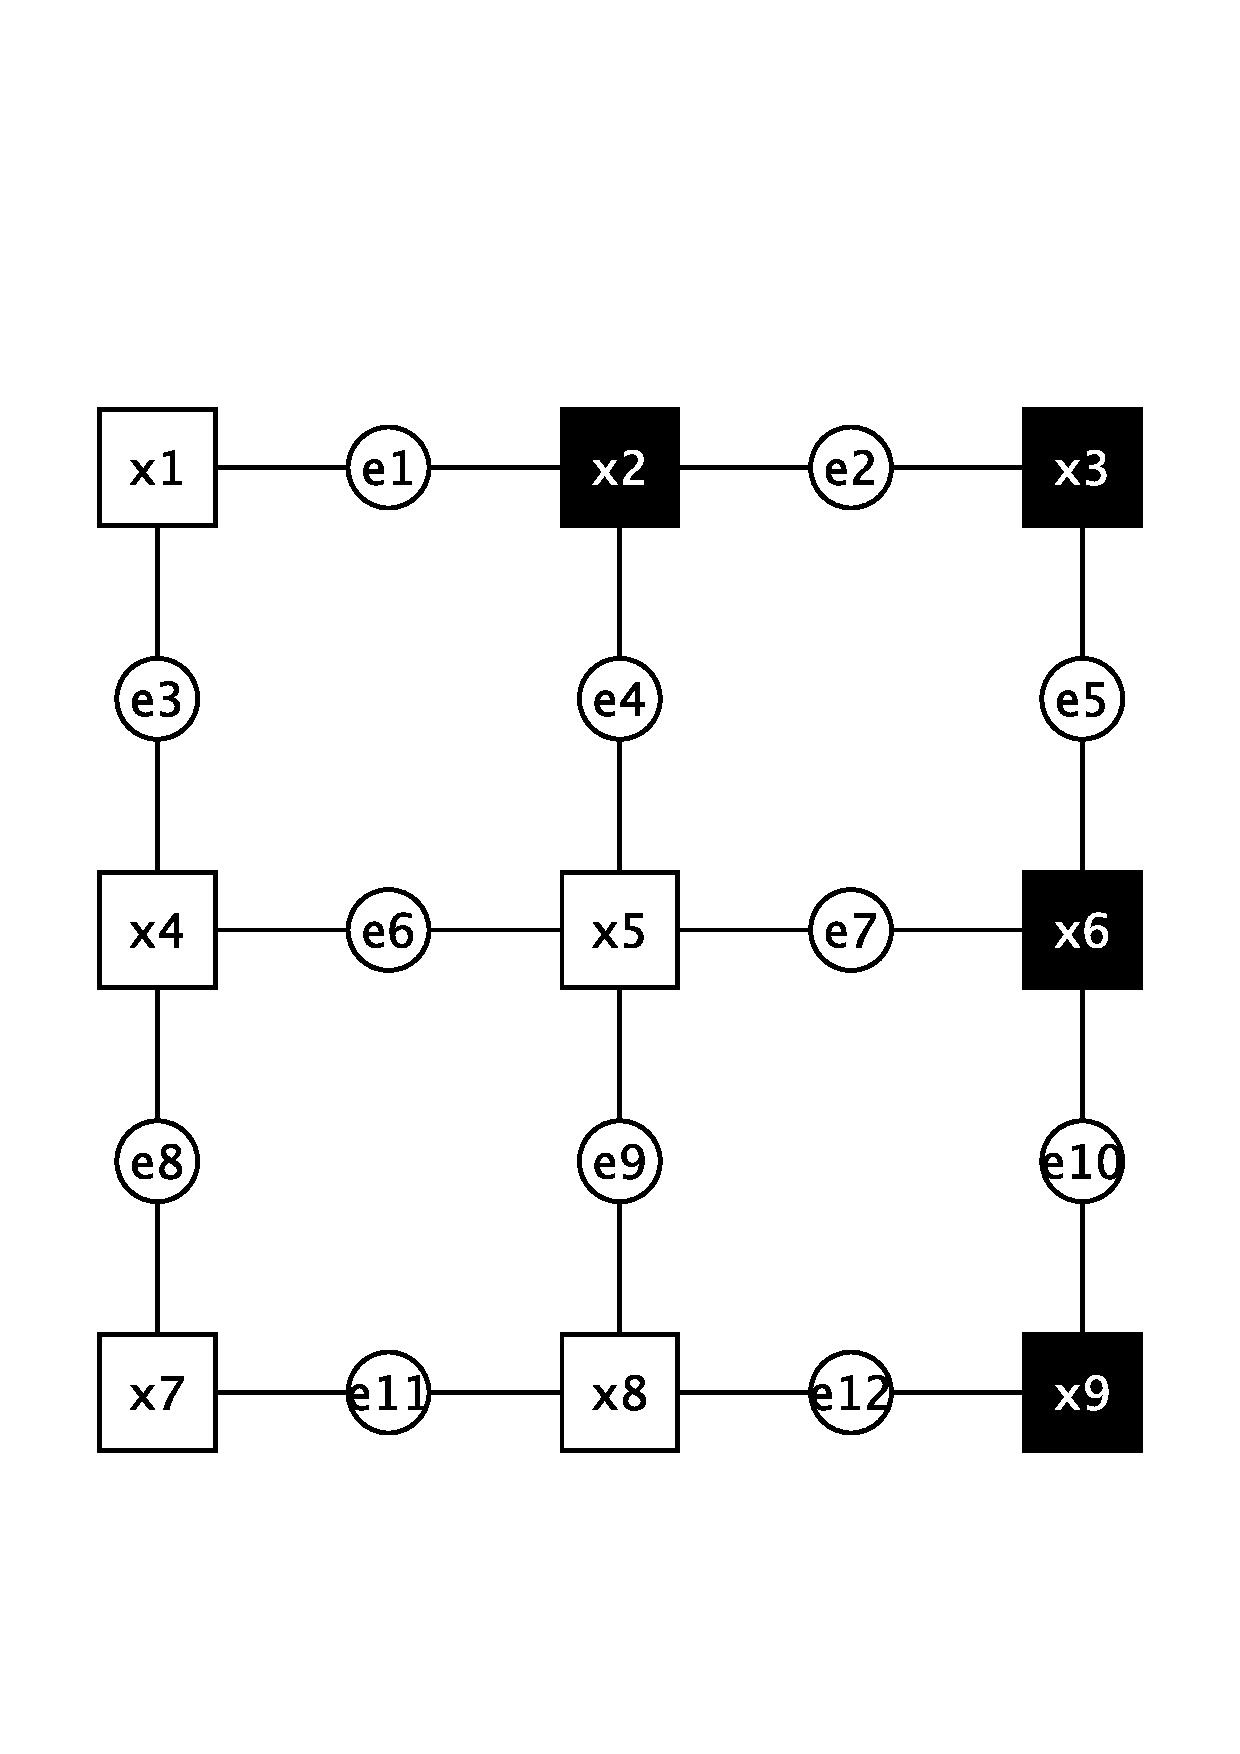
\includegraphics[scale=0.33]{mrfs.pdf}
\caption{Blocks as Nodes}
\label{fig:neighborhoods}
\end{figure}

Imagine we have a lattice of nine city blocks
$\{x_1,...x_9\}$. Between these blocks there are edges
$\{e_1,...,e_{12}\}$. Some of these blocks belong to the neighborhood
``Blacktown'' and other blocks belong to ``Whiteville'' (Figure
\ref{fig:neighborhoods}). 

Our task is try to learn something from this pattern of assignments
that we can use in another city. In particularly, we want to decide
what parts of a this new city are likely to belong to the same
neighborhood.

Since another city won't have a neighborhood called Whiteville or
Blacktown, learning about the qualities of these particular
neighborhoods won't be useful.

Instead, we'll try to learn where boundaries between neighborhoods are
likely to arise. 

First, we can construct a graph of our 12 edges where each ``edge
node'' now is either assigned to be a ``boundary edge'' or not. We
will add in some smoothing factors $\{f_1,...,f_{30}\}$ to encourage
contiguous boundaries (Figure \ref{fig:edges}).

\begin{figure}
\centering
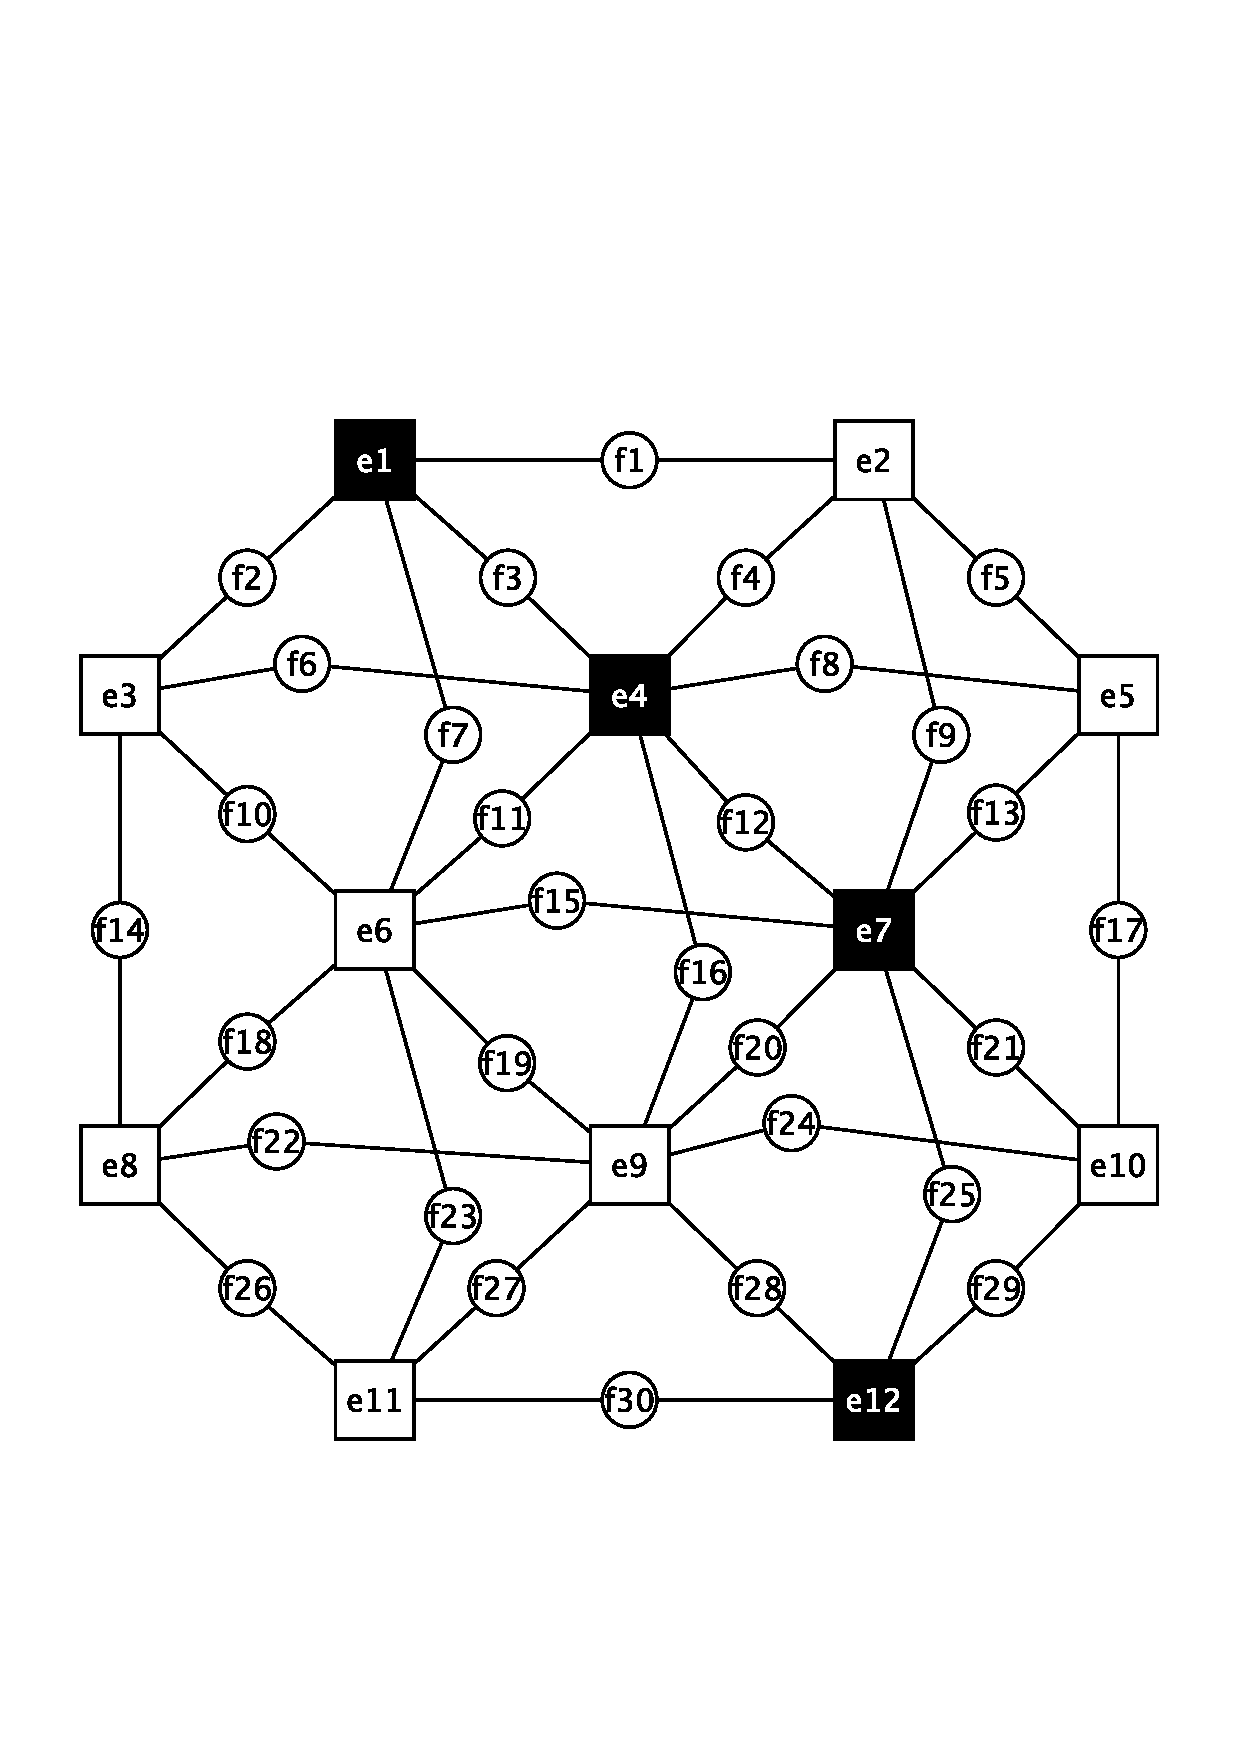
\includegraphics[scale=0.33]{edges.pdf}
\caption{Edges as Nodes, Black Nodes are ``boundary edges''}
\label{fig:edges}
\end{figure}

This boundary graph is an MRF, and we can write down the probability of boundary assignments as 

\begin{equation}
\Pr(X) = \frac{1}{Z}\operatorname{exp}(\sum_i\epsilon_i(e_i) + \sum_{<i j>}\epsilon_{i,j}(e_i,e_j)) 
\end{equation}

Where $j \in <i j>$ are all the edges that are neighbors of edge $i$.

Our task now is to try to learn the functions $\epsilon_i$ and
$\epsilon_{i,j}$. In our notional example, Blacktown is a low crime
area while Whiteville has more crime. Maybe neighborhood boundaries
are more likely to occur where there is large difference in crime
between city blocks.

We can encode that idea in the following form for $\epsilon_i$

\begin{equation}
\epsilon_i = \operatorname{logit^{-1}}(w_0 + w_1\operatorname{Similarity}(\text{Crime}_k, \text{Crime}_l))
\end{equation}

Where $k$ and $l$ are the city blocks separated by edge $i$. If this is an adequate model, all we need to do is find optimum weights $w_0, w_1$ and a good form for $\epsilon_{i,j}$.

\subsection*{Data}

I have a nightly updated database of geocoded Craigslist apartment
rentals, sublet, and roommate listings. For most of these listings,
the poster entered some text in the ``Specific Location'' field. With
some minimal pre-processing, we can use these data as observations of
claims that geographical points are in some neighborhood.

By using kernel density estimation for each neighborhood, we can use
this point data to estimate a continuous probability distributions
that any point in the city will be claimed to be in any of the
neighborhoods (Figure \ref{fig:KDE}.

\begin{figure}
\includegraphics{/home/fgregg/sweave-cache/figs/fig-KSplot.pdf}
\caption{KDE probability estimates of neighborhood claims on North Side}
\label{fig:KDE}
\end{figure}

However, KDE and other smoothers are... smooth. The estimates may
converge to true probability estimates as the amount of data
increases, but in the meantime these methods will produce overly
smooth decision boundaries between neighborhoods. 

We can correct for these artifacts if we have valid prior beliefs
about what kind of geographical features are likely to divide
neighborhoods. For example, we might believe that major roads, the
river, and railroad embankments are more likely to divide
neighborhoods than residential streets. 

We can encode these beliefs in the following model

\begin{equation}
\Pr(Y) = \frac{1}{Z}\operatorname{exp}\left(\sum_{<i j>}\epsilon_{i,j}(\text{Name}_i,\text{Name}_j) + \sum_i\epsilon_i(\text{Name}_i)\right) 
\end{equation}

Where $Y$ is a configuration of neighborhood names over census blocks,
$i$ indexes census blocks and the function $\epsilon_{i,j}$ has the
following form (blocks count as neighbors if they share any edge).

\begin{equation}
\epsilon_{i,j}(\text{Name}_i,\text{Name}_j) = \begin{cases}
  0 \quad\quad \text{Name}_i = \text{Name}_j \\
  0 \quad\quad \text{if $i$, $j$ are separated by a feature} \\
  \lambda \quad R_i \neq R_j \text{and not separated}
\end{cases}
\end{equation}

$\epsilon_i$ is just the estimated probabilities that a block $i$ will
be claimed to belong to a neighborhood for every neighborhood in the
city. This comes from calculating the densities kde estimates at the
centroid of a census block.

Entering these edge weights into our model, we can get a better estimate of
the boundaries between Chicago neighborhoods (Figure \ref{fig:graphcut}).

\begin{figure}
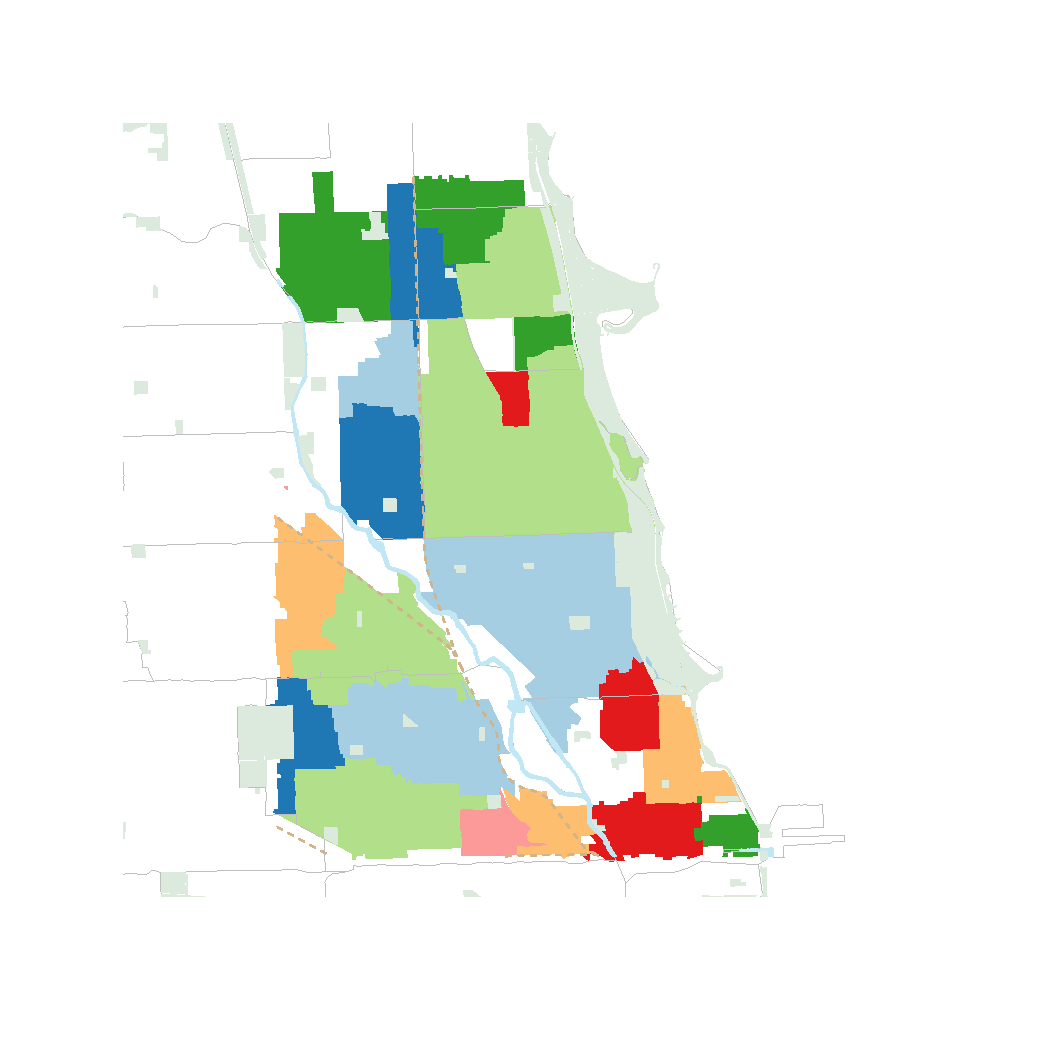
\includegraphics{respect_grid.pdf}
\caption{MAP estimate of neighborhood labels}
\label{fig:graphcut}
\end{figure}

These boundaries are our decisions boundaries. We have crime data for
every city block from the City of Chicago which we can enter into our
$\epsilon_i$. 

I also have the same kind of Craigslist data and social data for 50 of
the largest American cities.


\end{document}